\newgeometry{top=1cm, bottom=2cm}
\section{Determinante}
\begin{figure}[h!]
    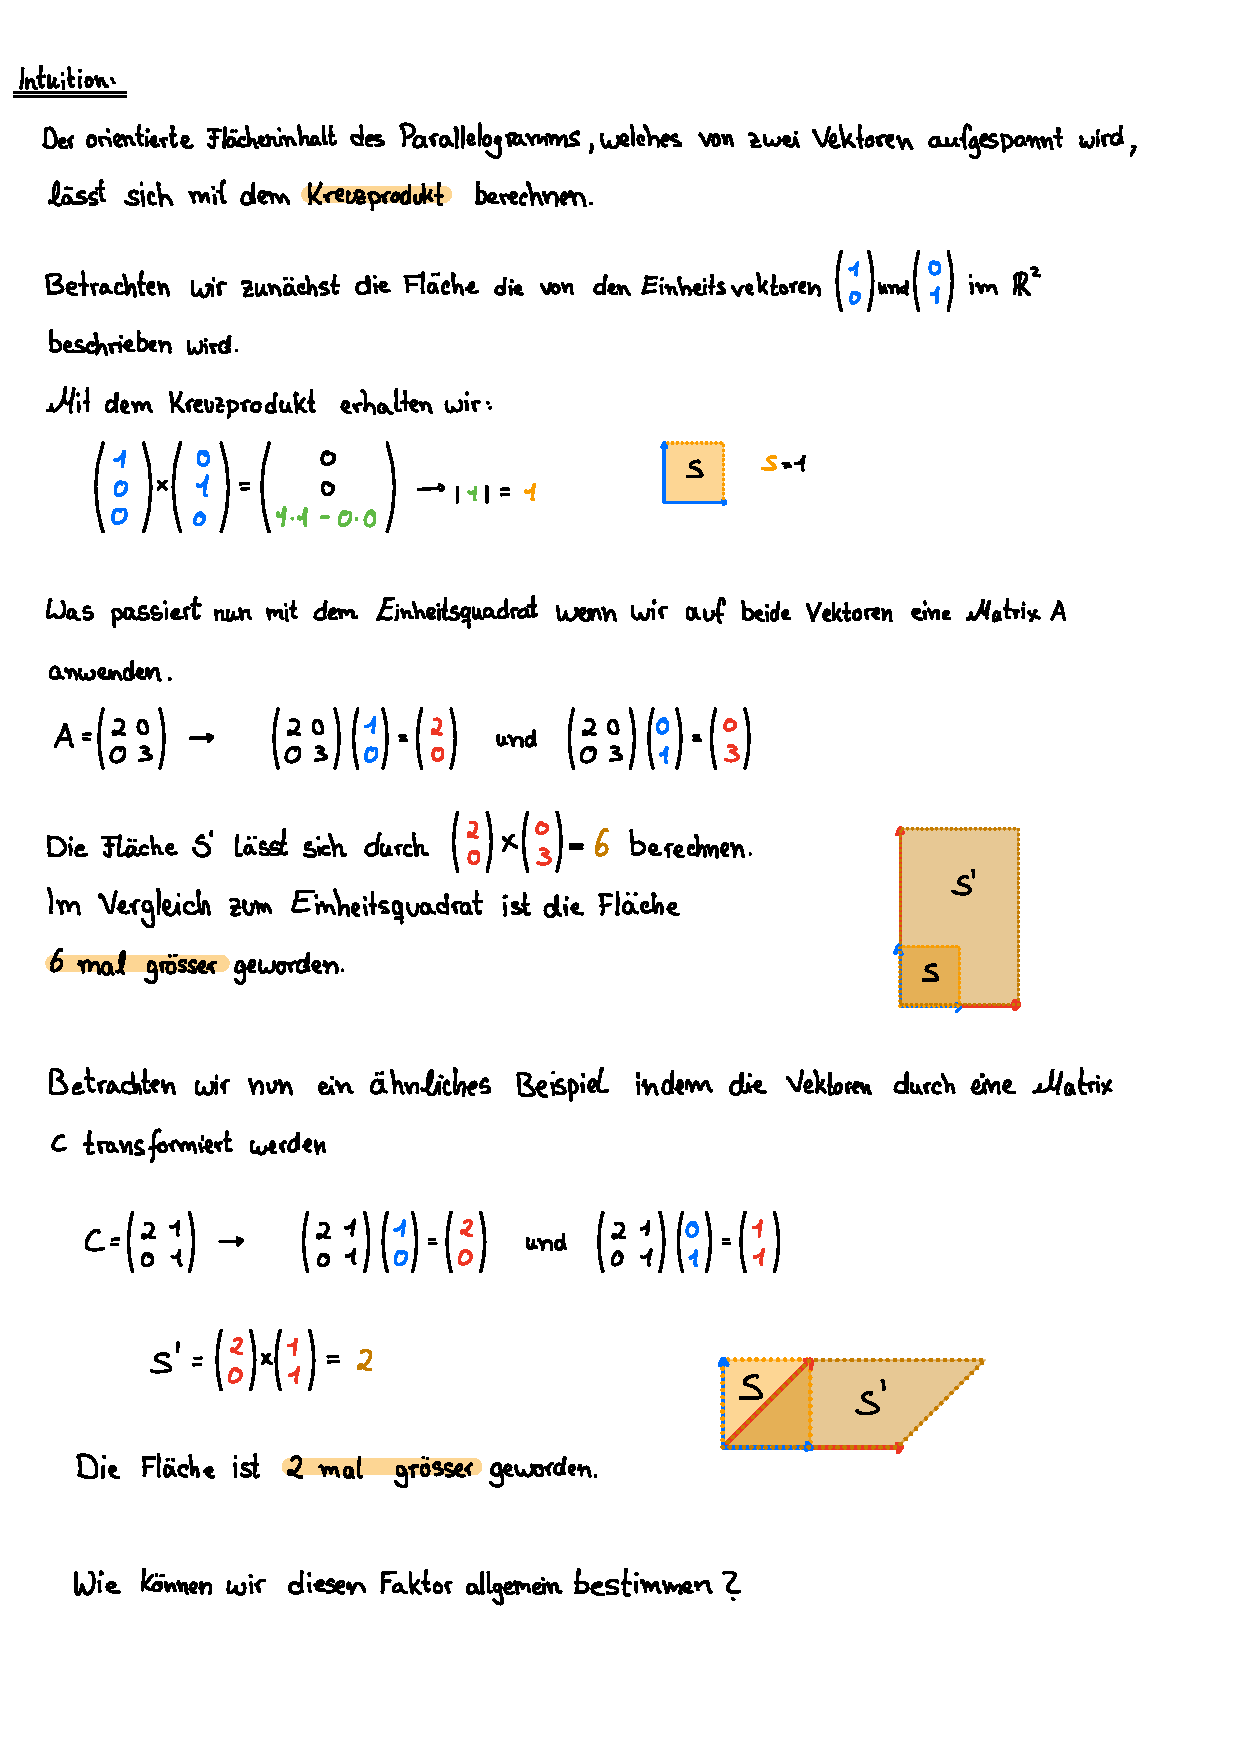
\includegraphics[page=1, scale=0.842]{pdf/03_Determinante.pdf}
\end{figure}
\newpage
\includepdf[pages={2-}, 
            pagecommand={\thispagestyle{plain}}, 
            scale=0.95]{pdf/03_Determinante.pdf}

\newgeometry{top=2.5cm, bottom=2cm}
\subsection{Beispielaufgaben} 
\vspace{1cm}
\subsubsection{} % Zardini S. 36
Sei
\[
A = \begin{pmatrix}
1 & 4 & 8 \\
3 & 4 & 6 \\
2 & 1 & 1 \\
\end{pmatrix}
\]
Berechne $det(A^\top)$. \\

\noindent \textbf{Lösung:}
\vspace{6cm}

\subsubsection{}
Sei \[
A = \begin{pmatrix}
1 & 2 \\
3 & 4 \\
\end{pmatrix}
\]
Berechne $det(A^{-1})$. \\

\noindent \textbf{Lösung:}

\newpage
\subsubsection{} %Zardini S. 42
Seien $a, b, c, d \in \mathbb{R}$ und
\[
M = \begin{pmatrix}
a & 0 & 0 & 0 & 0 & 0 \\
1 & -2 & 0 & -1 & 0 & 0 \\
2 & b & 0 & 3 & 0 & 0 \\
0 & 7 & 1 & -2 & 0 & 0 \\
-1 & 4 & 0 & 7 & -1 & c \\
5 & 1 & d & 4 & 1 & 2 \\
\end{pmatrix}.
\]
\begin{enumerate}[label=\alph*)]
    \item Berechnen Sie $det(M)$
    \item Für welche $a, b, c, d$ ist $M$ singulär?
\end{enumerate}

\noindent \textbf{Lösung:}

\newpage
\subsubsection{}%Zardini S. 51
Seien $a, b, c, d \in \mathbb{R}$ und
\[
A = \begin{pmatrix}
a & b & c & d \\
-3a & 2b & 3c & 2d \\
a & b & -c & d \\
-2a & -2b & -2c & d \\
\end{pmatrix}.
\]
Berechnen Sie die Determinante von $A$. \\

\noindent \textbf{Lösung:}

\newpage
\subsubsection{}
Seien $a, b, c, d \in \mathbb{R}$ und
\[
A = \begin{pmatrix}
a & b & c & d & b & b & d \\
b & c & d & d & b & d & a \\
c & d & b & c & d & c & c \\
d & b & c & d & b & b & c \\
b & d & c & b & d & b & b \\
b & c & d & d & b & d & a \\
d & a & c & d & a & b & c \\
\end{pmatrix}.
\]
Berechnen Sie die Determinante von $A$. \\

\noindent \textbf{Lösung:}
